
\section{Convolutional Tensor Compression}\label{sec:approx_tech}
%In typical object recognition architectures, the weights of
%convolutional layers at the end of training exhibit strong redundancy
%and regularity across all dimensions. 
In this section we describe
techniques for compressing 
4 dimensional convolutional weight tensors and fully connected weight matrices into a representation that permits
efficient computation and storage. 
Section \ref{reconstr_sect} describes how to construct a good approximation 
criteria. Section \ref{subsec:low_rank} describes techniques for low-rank tensor
approximations. Sections \ref{subsec:monochromatic} and \ref{subsec:clustering} describe how to 
apply these techniques to approximate weights of a convolutional neural network.
%and Section \ref{finetuningsect}
%explains the fine-tuning strategy used in experiments.
%Section  shows how to use clustering algorithms to
%discover, and later exploit, patterns between input and output
%features.

% \vspace{2mm}

%\vspace{-0.3cm}

%\section{Application to Convolutional Networks}\label{sec:application}

%In this section we describe how to use the techniques described in
%Section \ref{sec:approx_tech} to approximate covolutional weight
%tensors in ways that allow for a more efficient computation of the
%convolution. The approximations are more efficient in two aspects:
%both the number of floating point operations required to compute the
%convolution output and the number of parameters that need to be stored
%are dramatically reduced.

\subsection{Approximation Metric}
\label{reconstr_sect}

The goal is to find an approximation $\tilde{W}$ of a convolutional tensor $W$ 
that facilitates more efficient computation while maintaining the prediction performance of the network.
A natural choice for an approximation criterion is
to minimize $\| \tilde{W} - W \|_F$. This criterion yields 
efficient compression schemes using elementary linear algebra, and also controls
the operator norm of each linear convolutional layer.
%
%Euclidean distance has the advantage that then finding low-rank 
%approximations can be solved explicitly with efficient algorithms. 
However, this criterion assumes that all directions in the space of weights equally 
affect prediction performance. We now present two methods of improving this criterion while 
keeping the same efficient approximation algorithms.

{\bf Mahalanobis distance metric: }
The first distance metric we propose seeks to emphasize coordinates more prone to produce prediction errors over 
coordinates whose effect is less harmful for the overall system. 
We can obtain such measurements as follows.
Let $\Theta=\{W_1,\dots,W_S\}$ denote
Let $\Theta=\{W_1,\dots,W_S\}$ denote
the set of all parameters of the $S$-layer network, and let $U(I; \Theta)$ denote the output 
after the softmax layer of input image $I$.
We consider  a given input training set $(I_1,\dots,I_N)$ 
with known labels $(y_1,\dots,y_N)$. For each pair $(I_n, y_n)$, 
the compute the forward propagation pass $U(I_n, \Theta)$, and 
define as $\{\beta_n\}$ the indices of the $h$ largest values of  $U(I_n, \Theta)$ 
different from $y_n$.
Then, for a given layer $s$, we compute
\begin{equation}
\label{approxi}
d_{n,l,s} = \nabla_{W_s} \left( U(I_n, \Theta) - \delta(i - l)\right)~,~n\leq N\,,\, l \in \{\beta_n\}\,,\, s\leq S~,
\end{equation}
where $\delta(i-l)$ is the dirac distribution centered at $l$.
In other words, for each input we back-propagate the difference between the current prediction and the 
$h$ ``most dangerous" mistakes. 

The Mahalanobis distance is defined from the covariance of 
$d$: $\| W \|_{maha}^2 = w \Sigma^{-1} w^T~,$
where $w$ is the vector containing all the coordinates of $W$, and $\Sigma$ is the covariance of $(d_{n,l,s})_{n,l}$. 
We do not report results using this metric, since it requires inverting a matrix of size equal to the number 
of parameters, which can be prohibitively expensive in large networks.
Instead we use an approximation that considers only the diagonal of the covariance matrix. 
In particular, we propose the following, approximate, Mahalanobis distance metric: 
\begin{equation}
\label{poormansmaha}
\| W \|_{\widetilde{maha}} := \sum_p \alpha_p W(p) ~,\text{ where } \alpha_p = \Big( \sum_{n,l} d_{n,l,s}(p)^2 \Big)^{1/2}~
\end{equation}
where the sum runs over the tensor coordinates.
Since (\ref{poormansmaha}) is a reweighted Euclidiean metric, we 
can simply compute $W' = \alpha~ .* W$, where $.*$ denotes element-wise multiplication, 
then compute the approximation $\widetilde{W'}$ on $W'$ using the standard $L_2$ norm, 
and finally output $\widetilde{W} = \alpha^{-1} .* \widetilde{W'}~.$

{\bf Data covariance distance metric: }
One can view the Frobenius norm of $W$ as
$\| W \|_F^2 = \mathbb{E}_{x \sim \mathcal{N}(0,I)} \| W x \|_F^2 ~.$
Another alternative, which has also been considered in \cite{zisserman14}, is to replace the isotropic covariance
assumption by the empirical covariance of the input of the layer. If $W \in \mathbb{R}^{C \times X \times Y \times F}$ 
is a convolutional layer, and $\widehat{\Sigma} \in \mathbb{R}^{CXY \times CXY}$ is the empirical estimate of the input data covariance, 
it can be efficiently computed as 
\begin{equation}
\| W \|_{data} = \| \widehat{\Sigma}^{1/2} W_F \|_F~, 
\end{equation}
where $W_F$ is the matrix obtained by folding the first three dimensions of $W$.

%Figure \ref{fig:components} compares the relationship between reconstruction error and prediction error 
%using the unweighted and reweighted distance metrics, measured on
%$4096$ samples of Imagenet for a range of different approximation hyperparameters.
% As expected, the reweighted $L_2$ distance correlates more strongly with
% performance loss. Consequently, optimizing the reweighted distance
% reduces the performance drop, for a given $\ell_2$ reconstruction error.
%
%\begin{figure}[h]
%\centering
%\begin{minipage}{0.75\textwidth}
%  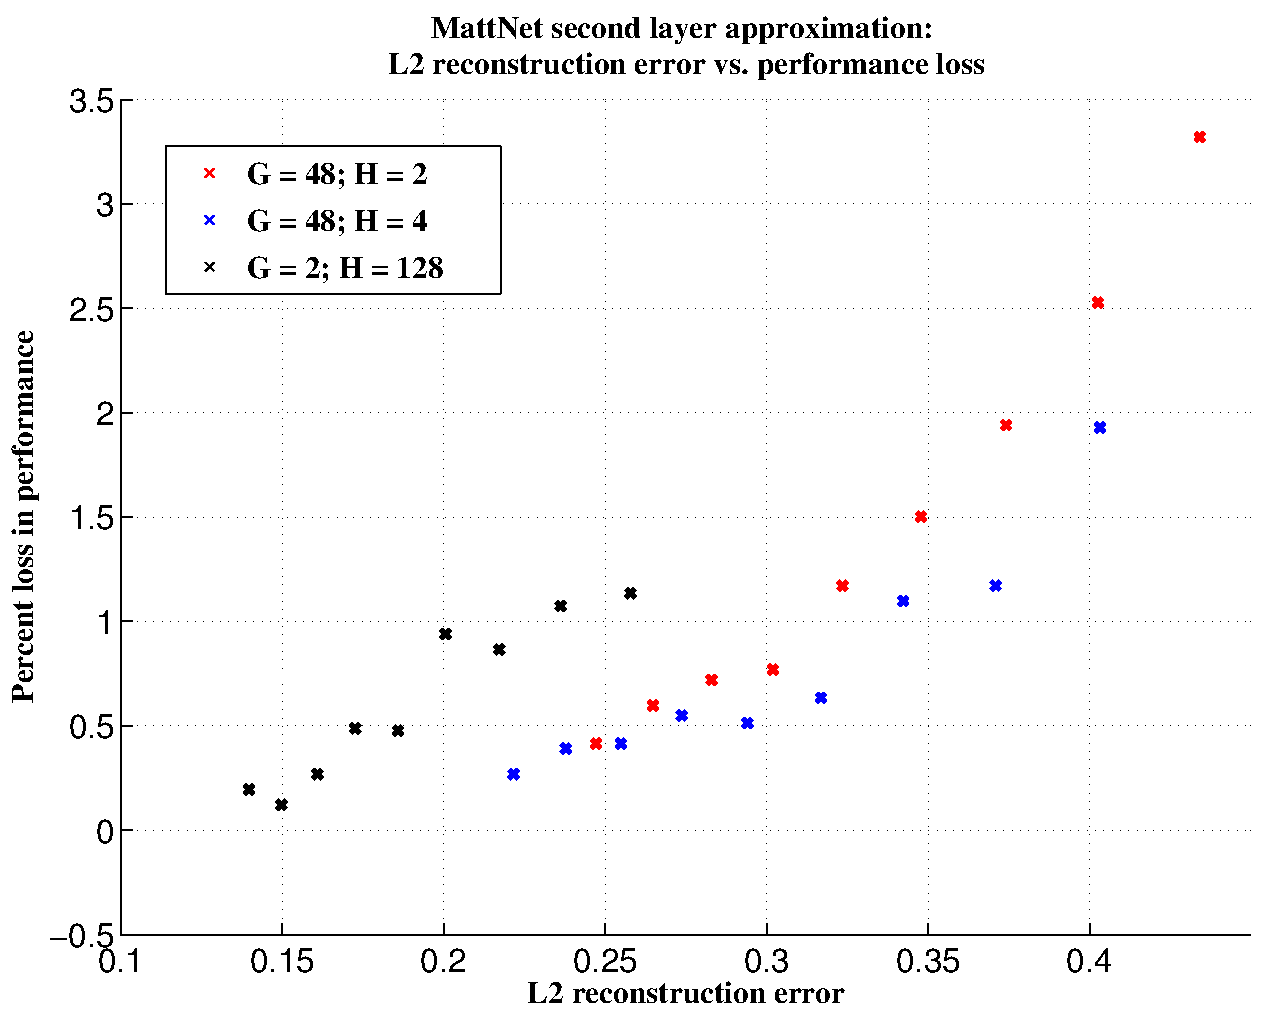
\includegraphics[width=0.5\linewidth]{img/biclustering_L2_vs_testerr_matt.pdf} 
%\quad\quad
%  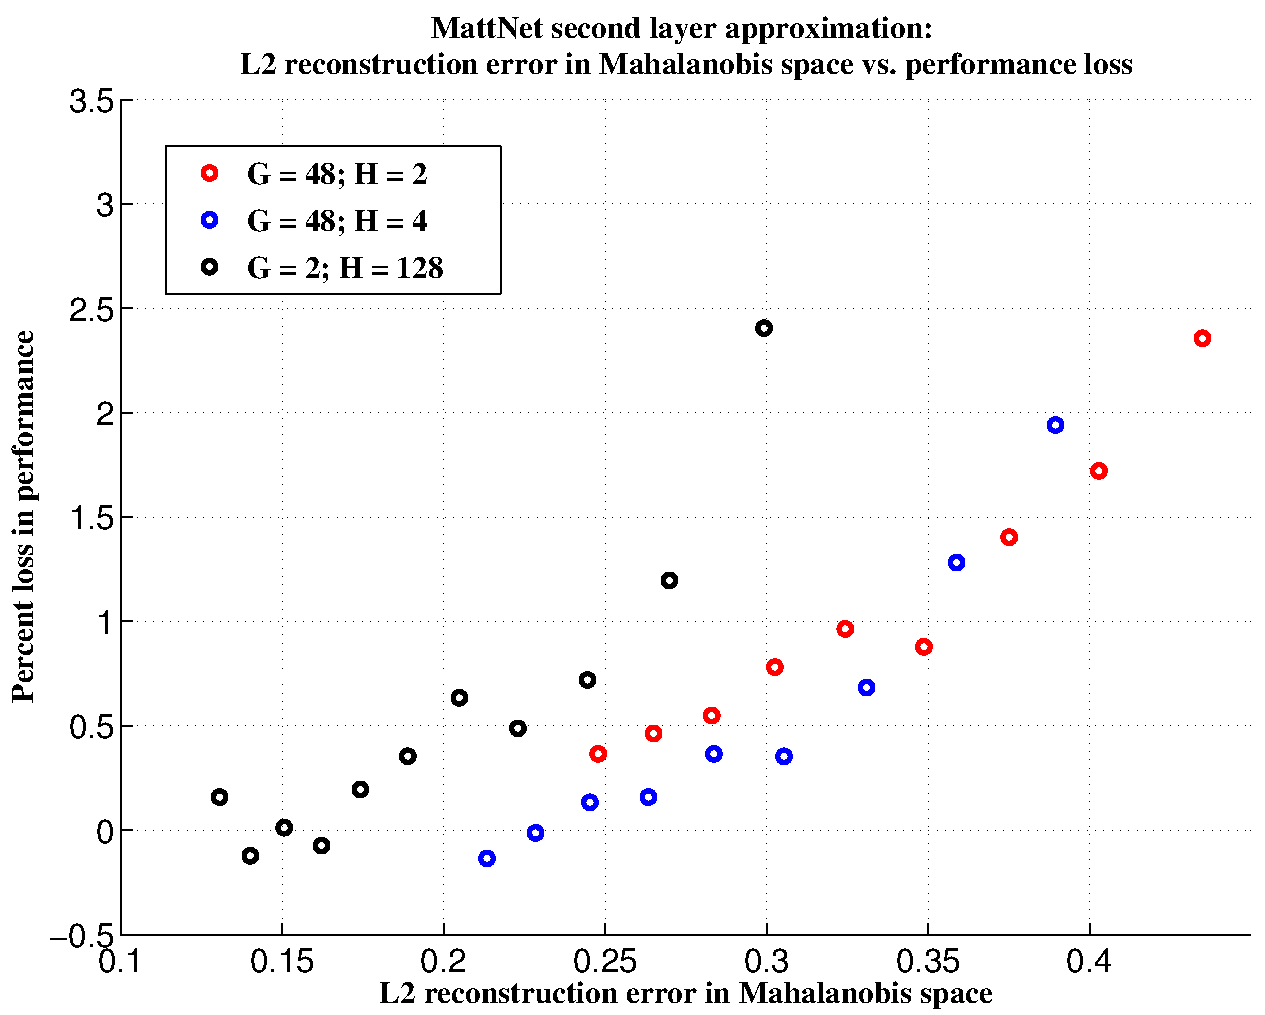
\includegraphics[width=0.5\linewidth]{img/biclustering_L2_vs_testerr_maha_matt.pdf} 
%\end{minipage}
%\vspace{-3mm}
%\caption{$\ell_2$ reconstruction error of approximated weights in the
%  original space (left) and the reweighted space (designed to match
%  output error, see
%  \ref{poormansmaha}) (right), versus decrease in peformance for a
%  range of different approximation hyperparameters. Markers with the
%  same color use the same settings for $G,H$ but vary the
%  approximation rank. The reweighted space makes the correlation
%  between $l_2$ and classification error more linear (e.g.~the red
%  circles are well approximated by a line, but no so for the red
%  crosses). Furthermore, for a given $l_2$ error, the performance loss
%  is lower for the reweighted space. }
%\label{fig:components}
%\end{figure}
%

%\subsection{kk}\label{subsec:monochromatic}

\subsection{Low-rank Tensor Approximations}\label{subsec:low_rank}

A particularly simple strategy to exploit the redundancy present in trained convolutional network weights is to 
linearly compress the tensors, which amounts to finding low-rank approximations. 
%In this section we describe two different techniques for expressing matrices and tensors as a product of matrices or vectors of smaller size. 

%\vspace{-0.3cm}
\subsubsection{Matrix Decomposition}\label{subsubsec:svd}
Matrices are $2$-tensors which can be linearly compressed using the Singular Value Decomposition. 
If $W \in \mathbb{R}^{m \times k}$ is a real matrix, the SVD is defined as
%\begin{equation*}
	$W = USV^{\top}$, where $U \in \mathbb{R}^{m \times m}, S \in \mathbb{R}^{m \times k}, V \in \mathbb{R}^{k \times k}$.
%\end{equation*}
$S$ is a diagonal matrix with the singular values on the diagonal, and $U$, $V$ are orthogonal matrices. 
If the singular values of $W$ decay rapidly, $W$ can be well approximated by keeping only the $t$ largest entries of $S$, 
resulting in the approximation 
%We can write the approximation as
%\begin{equation}
%\label{svdapprox}
	$\tilde{W} = \tilde{U}\tilde{S}\tilde{V}^{\top}$, where $\tilde{U} \in \mathbb{R}^{m \times t}, \tilde{S} \in \mathbb{R}^{t \times t}, \tilde{V} \in \mathbb{R}^{t \times k}$
%\end{equation}
Then, for $I \in \mathbb{R}^{n \times m}$, the approximation error $\| I \tilde{W} - I W \|_F$ satisfies 
%\begin{equation}
%\label{svdapproxerr}
  $\| I \tilde{W} - I W \|_F \leq s_{t+1} \| I \|_F~,$
%\end{equation}
and thus is controlled by the decay along the diagonal of $S$.
Now the computation $I\tilde{W}$ can be done in $O(nmt + nt^2 + ntk)$, which, for sufficiently small $t$ is significantly smaller than $O(nmk)$. 

%\vspace{-0.3cm}
%\subsubsection{Low Rank Tensor Approximations}\label{subsubsec:svd_tensor}
\subsubsection{Higher Order Tensor Approximations}\label{subsubsec:svd_tensor}
SVD can be used to approximate a tensor $W \in \mathbb{R}^{m \times n \times k}$
by first folding all but two dimensions together to convert it into a $2$-tensor, %eg $W_f \in \mathbb{R}^{m \times (n \cdot k)}$, 
and then considering the SVD of the resulting matrix. For example, we can approximate $W_m \in \mathbb{R}^{m \times (nk)}$ as $\tilde{W}_m \approx \tilde{U}\tilde{S}\tilde{V}^{\top}$. 
$W$ can be compressed even further by applying SVD to $\tilde{V}$. We refer to this approximation as the SVD decomposition and use $K_1$ and $K_2$ to denote the rank used in the first and second application of SVD respectively.
%For example, 
%%
%%Any tensor can be converted to a matrix by folding all but two
%%dimensions together.  For example, 
%let $W_C \in \mathbb{R}^{C \times (XYF)}$ be a folded version of a convolutional $4$-tensor $W$, where the spatial and output dimensions have been folded together. The Singular value decomposition of
%$W_C$ can decrease number of input colors on which the convolution has to
%operate in exchange for an additional matrix multiplication
%operation. More formally, $$W_C = USV^T \approx
%\tilde{U}\tilde{S}\tilde{V}^T~,$$
%where $\tilde{U}\tilde{S}$ is a matrix that
%transforms input colors to an intermediate output.  Then $\tilde{V}$ is
%considered as a convolution operator on intermediate output space. 
%Similarly, we can apply the SVD to $W_F \in \mathbb{R}^{(CXY) \times F}$ or $\tilde{V}$. 

%\vspace{-0.3cm}
%\subsubsection{Outer Product Decomposition for Tensors:}\label{subsubsec:outer}
Alternatively, we can approximate a 3-tensor, $W_S \in \mathbb{R}^{m \times n \times k}$, by a rank 1 3-tensor by finding a decomposition that minimizes 
\begin{equation}
\label{eq:rank1}
	\| W - \alpha \otimes \beta \otimes \gamma \|_F~,
\end{equation} 
where $\alpha \in \mathbb{R}^m$, $\beta \in \mathbb{R}^{n}$, $\gamma \in \mathbb{R}^k$ and $\otimes$ denotes the outer product operation.
Problem (\ref{eq:rank1}) is solved efficiently by performing alternate least squares 
on $\alpha$, $\beta$ and $\gamma$ respectively, although more efficient algorithms can also be 
considered \cite{rankonetensors}. 

This easily extends to a rank $K$ approximation using a greedy algorithm: Given a 
tensor $M$, we compute $(\alpha, \beta, \gamma)$ using (\ref{eq:rank1}), and we update 
$W_S \leftarrow W_S - \alpha \otimes \beta \otimes \gamma$. Repeating this operation $K$
times results in 
\begin{equation}
\label{eq:rankK}
	\tilde{W_S} = \sum_{k = 1}^{K} \alpha_k \otimes \beta_k \otimes \gamma_k ~.
\end{equation} 
We refer to this approximation as the outer product decomposition ans use $K$ to denote the rank of the approximation.

%\subsection{Clustering}\label{subsec:clustering}
%Another form of structure within the 4-D weight tensors that can be exploited is the similarity between different filters. 
%We can capture this by first splitting the filters into groups and then approximating the weights within a group using a low-rank factorization method.  
%We found it to be most efficient to independently cluster
%over both input and output feature channels. We start by clustering the
%rows of $W_C \in \mathbb{R}^{C \times (XYF)}$, which results in
%clusters $C_1, \dots, C_a$. Then we cluster the columns of $W_F  \in
%\mathbb{R}^{(CXY) \times F}$. This procedure returns clusters $F_1,
%\dots, F_b$. These two operations break the original weight tensor $W$
%into $ab$ sub-tensors $\{W_{C_i, F_j}\}_{i = 1, \dots, a, j = 1,
%  \dots, b}$ as shown in Figure \ref{fig:biclustering}). Each
%sub-tensor contains similar elements making this approach more
%efficient than attempting to fit a low rank approximation to all
%filters.
%
%In order to efficiently exploit the parallelism inherent in CPU and GPU
%architectures it is useful to constrain clusters to be of equal sizes. 
%We therefore perform the biclustering operations (or clustering 
%for monochromatic filters \ref{subsec:monochromatic}) using a modified
%version of the k-means algorithms which balances the cluster count at
%each iteration
%It is implemented with the Floyd algorithm, by modifying the Euclidean distance
%with a subspace projection distance.

%The first convolutional layer in the standard architecture receives
%three color channels, typically in RGB or YUV space, as input whereas
%later hidden layers typically receive a much larger number of feature
%maps that have resulted from computations performed in previous
%layers. As a result, the first layer weights often have a markedly
%different structure than the weights in later convolutional layers. We
%have found that different approximation techniques are well suited to
%the different layers. The first approach, which we call {\em monochromatic
%approximation}, can be applied to the weights in the first
%convolutional layer. For the remaining layers, where the number of
%input and output maps are large, we use the 
%biclustering approximation, outlined in Section
%\ref{subsubsec:biclustering}.

%We will compare the number of floating-point operations for different
%approximation methods. Table \ref{table:ops} shows a breakdown of the number of operations required for the standard convolution and for our approximations.
%\subsection{Clustering}\label{subsec:clustering}
%Another form of structure within the 4-D weight tensors that can be exploited is the similarity between different filters. 
%We can capture this by first splitting the filters into groups and then approximating the weights within a group using a low-rank factorization method.  
%We found it to be most efficient to independently cluster
%over both input and output feature channels. We start by clustering the
%rows of $W_C \in \mathbb{R}^{C \times (XYF)}$, which results in
%clusters $C_1, \dots, C_a$. Then we cluster the columns of $W_F  \in
%\mathbb{R}^{(CXY) \times F}$. This procedure returns clusters $F_1,
%\dots, F_b$. These two operations break the original weight tensor $W$
%into $ab$ sub-tensors $\{W_{C_i, F_j}\}_{i = 1, \dots, a, j = 1,
%  \dots, b}$ as shown in Figure \ref{fig:biclustering}). Each
%sub-tensor contains similar elements making this approach more
%efficient than attempting to fit a low rank approximation to all
%filters.
%
%In order to efficiently exploit the parallelism inherent in CPU and GPU
%architectures it is useful to constrain clusters to be of equal sizes. 
%We therefore perform the biclustering operations (or clustering 
%for monochromatic filters \ref{subsec:monochromatic}) using a modified
%version of the k-means algorithms which balances the cluster count at
%each iteration
%It is implemented with the Floyd algorithm, by modifying the Euclidean distance
%with a subspace projection distance.
%
%\section{Application to Convolutional Networks}\label{sec:application}
%In this section we describe how to use the techniques described in
%Section \ref{sec:approx_tech} to approximate covolutional weight
%tensors in ways that allow for a more efficient computation of the
%convolution. The approximations are more efficient in two senses:
%both the number of floating point operations required to compute the
%convolution output and the number of parameters that need to be stored
%are dramatically reduced.
%
%The first convolutional layer in the standard architecture receives
%three color channels, typically in RGB or YUV space, as input whereas
%later hidden layers typically receive a much larger number of feature
%maps that have resulted from computations performed in previous
%layers. As a result, the first layer weights often have a markedly
%different structure than the weights in later convolutional layers. We
%have found that different approximation techniques are well suited to
%the different layers. The first approach, which we call {\em monochromatic
%approximation}, can be applied to the weights in the first
%convolutional layer. For the remaining layers, where the number of
%input and output maps are large, we use the 
%biclustering approximation, outlined in Section
%\ref{subsubsec:biclustering}.
%
%We will compare the number of floating-point operations for different
%approximation methods. Table \ref{table:ops} shows a breakdown of the number of operations required for the standard convolution and for our approximations.

\begin{figure}[ht]
\centering
\mbox{
%\hspace{5mm}
\subfigure[][]{
  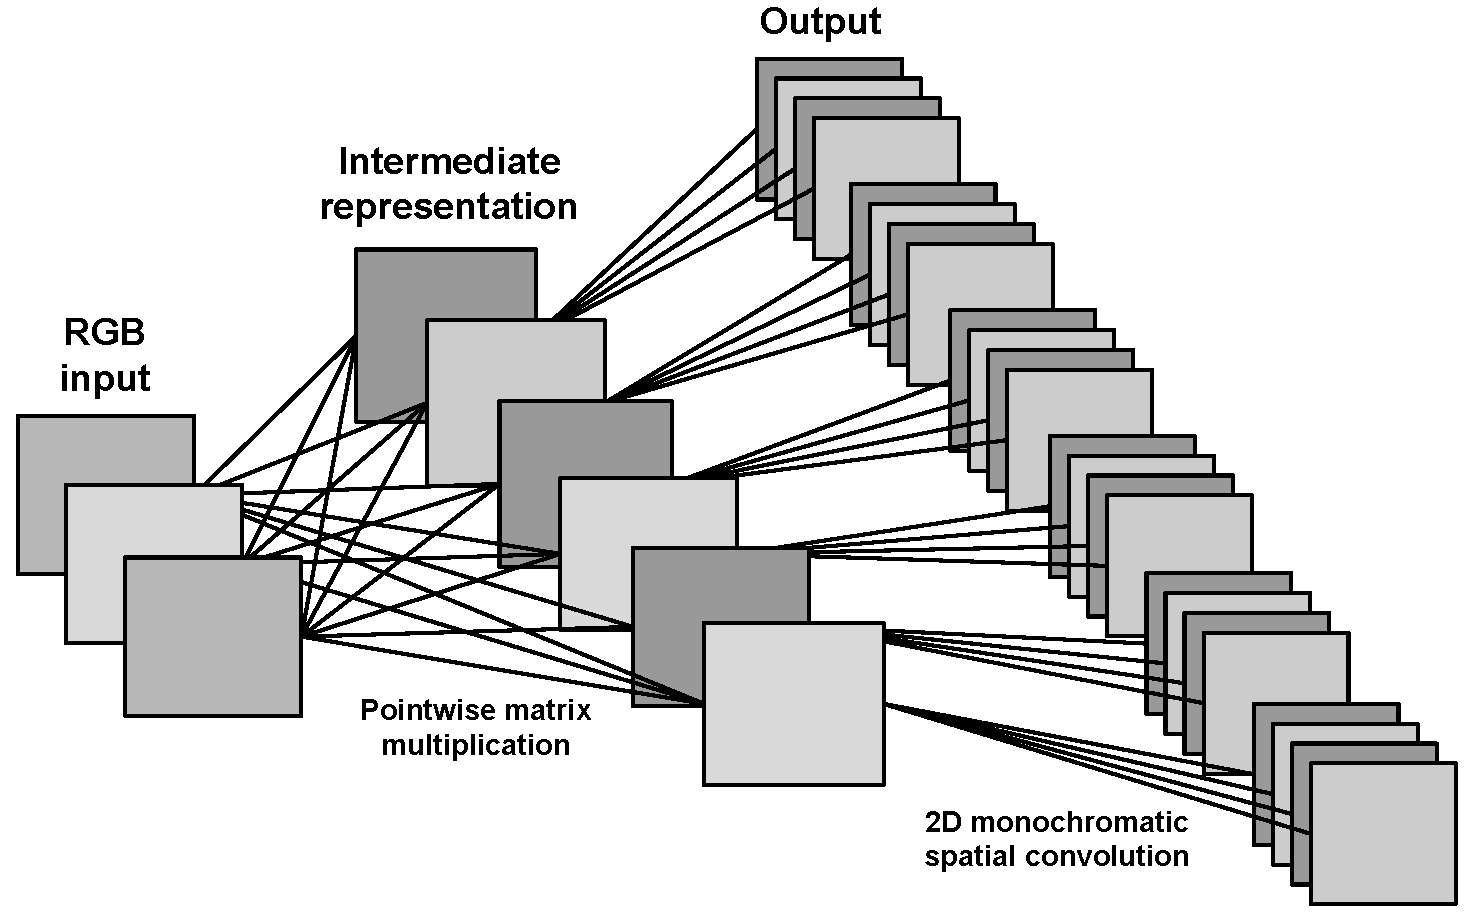
\includegraphics[width=0.3\linewidth]{img/monochromatic_illustration.pdf} 
  \label{fig:monochromatic}
}
\hspace{1mm}
\subfigure[][]{
  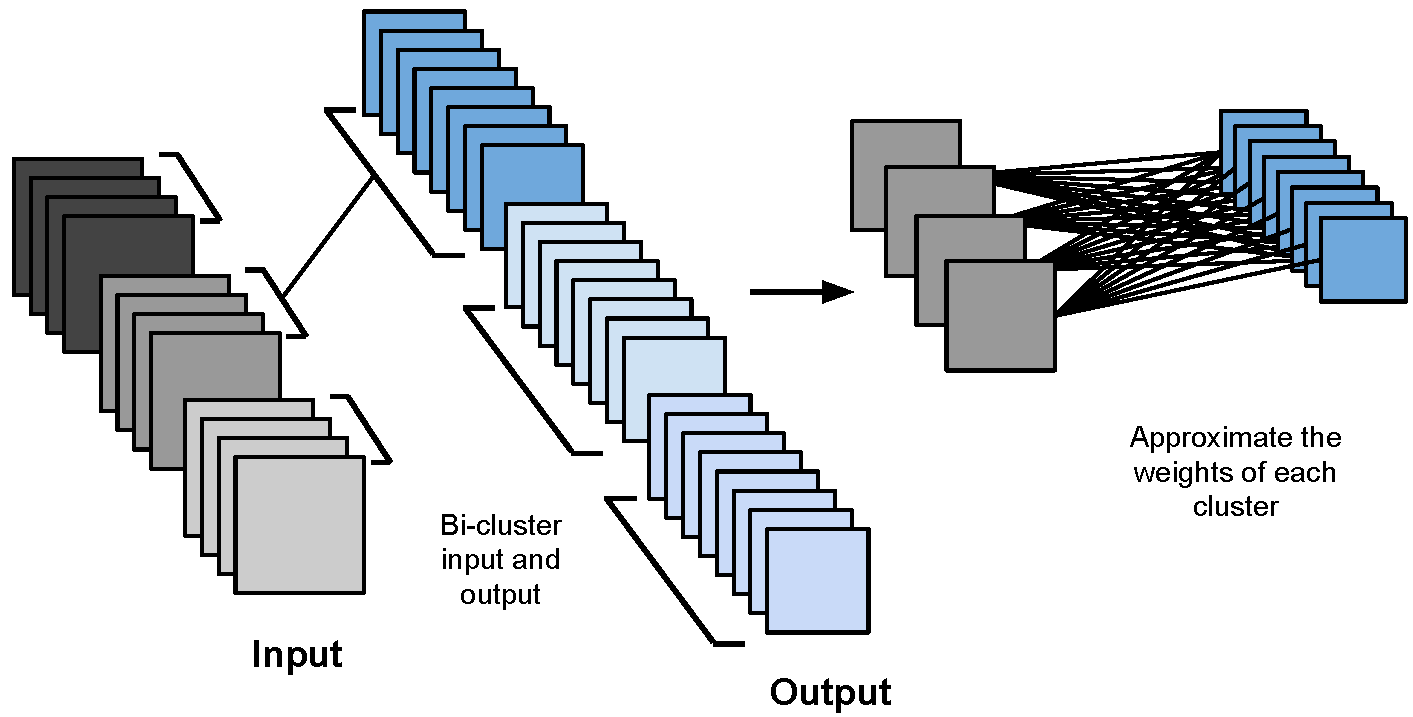
\includegraphics[width=0.3\linewidth]{img/bicluster_illustration.pdf} 
  \label{fig:biclustering}
}
\hspace{1mm}
\subfigure[][]{
  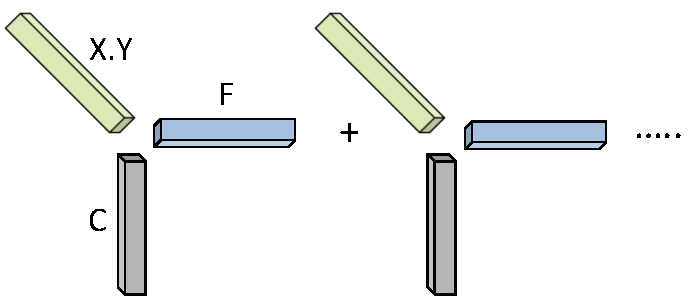
\includegraphics[width=0.3\linewidth]{img/tensor_sum.pdf} 
  \label{fig:monochromatic}
}
}
\vspace{-3mm}
\caption{ A visualization of monochromatic and biclustering approximation structures. {\bf (a)} The monochromatic approximation, used for the first layer. Input color channels are projected by a set of intermediate color channels. After this transformation, output features need only to look at one intermediate color channel. This sparsity structure is what makes the speedups feasible. {\bf (b)} The biclustering approximation, used for higher convolution layers. Input and output features are clustered into equal sized groups. The weight tensor corresponding to each pair of input and output clusters is then approximated. {\bf (c)} The weight tensors for each input-output pair in (b) is approximated by a sum of rank 1 tensors using techniques described in \ref{subsubsec:svd_tensor}}
\end{figure}

\subsection{Monochromatic Convolution Approximation}\label{subsec:monochromatic}
Let $W \in \mathbb{R}^{C \times X \times Y \times F}$ denote the
weights of the first convolutional layer of a trained network.  The
number of input channels, $C$, corresponds to a different color
component (either RGB or YUV).  
We found that the color components
tend to have low dimensional structure. In
particular, the weights can be well approximated by projecting the
color dimension down to a 1D subspace, i.e. a single color
channel. The low-dimensional structure of the weights is apparent in
\ref{fig:RGB_components} which shows the original first layer convolutional weights
and the weights after the color dimension has
been projected into 1D lines.

The monochromatic approximation exploits this structure and is computed as follows.
First, for every output feature, $f$, we consider consider the matrix $W_f \in \mathbb{R}^{C \times (XY) }$, 
where the spatial dimensions of the filter corresponding to the output feature have been combined, and find the SVD, 
$W_f = U_f S_f V_f^{\top}$,
%\begin{equation*}
%	W_f = U_f S_f V_f^{\top}
%\end{equation*}
where $U_f \in \mathbb{R}^{C \times C}, S_f \in \mathbb{R}^{C \times XY}$, and $V_f \in \mathbb{R}^{XY \times XY}$. 
We then take the rank $1$ approximation of $W_f$: 
\begin{equation}
\label{blo1}
	\tilde{W}_f = \tilde{U}_f \tilde{S}_f \tilde{V}_f^{\top} ~,
\end{equation}
where $\tilde{U}_f \in \mathbb{R}^{C \times 1}, \tilde{S}_f \in \mathbb{R}, \tilde{V}_f \in \mathbb{R}^{1 \times XY}$.
This approximation corresponds to using a single color channel for each output feature. 
We can further exploit the regularity in the weights by sharing the color component basis between different output features. 
We do this by clustering the $F$ left singular vectors, $\tilde{U}_f$, of each output feature $f$ into $C'$ clusters, 
where $C'$ is much smaller than $F$. We constrain the clusters to be of equal size as discussed in section \ref{subsec:clustering}.  
Then, for each of the $\frac{F}{C'}$ output features $f$ that is assigned to cluster $c_f$, we can approximate $W_f$ with
\begin{equation}
\label{blo2}
	\tilde{W}_f = U_{c_f} \tilde{S}_f \tilde{V}_f^{\top}
\end{equation}
where $U_{c_f} \in \mathbb{R}^{C \times 1}$ is the cluster center for cluster $c_f$ and $\tilde{S}_f$ and $\tilde{V}_f$ as as before. 


%By decomposing the approximated weights into two tensors, this low-rank approximation
% allows for a more efficient computation of the convolutional layer output. 
% Let $W_C \in \mathbb{R}^{C' \times C}$ denote the color transform matrix 
% where the rows of $W_C$ are the cluster centers $U_c^{\top}$. 
% Let $W_{mono} \in \mathbb{R}^{X \times Y \times F}$ denote the monochromatic 
% weight tensor containing $ \tilde{S}_f \tilde{V}_f^{\top}$ for each of the $F$ output features. 
% Given this decomposition, we can compute the output of the convolutional layer by first 
% transforming the input signal, $I \in \mathbb{R}^{C \times N \times M}$ into a different 
% basis using the color transform matrix: $\tilde{I} = W_C \otimes I$
% where $\tilde{I} \in \mathbb{R}^{C' \times N \times M}$. 
%
%After the color transformation (left part of the Figure \ref{fig:monochromatic}), 
%each of the $f$ filters in $W_{mono}$ is monochromatic in the sense that it only acts upon one of the $C'$ color channels 
%(right part of the Figure \ref{fig:monochromatic}). 
%The fact that this approximation can be made without hurting performance indicates that the 
%structure inherent in first layer weights inherently has sparsity
%between the input and output maps, when projected into the new color basis. 
%If the color transformation is computed once at the outset, then the
%number of operations performed is significantly reduced. 
This monochromatic approximation is illustrated in the left panel of Figure \ref{fig:monochromatic}.
Table \ref{table:ops} shows the number of operations required for the standard and monochromatic versions.

\subsection{Biclustering Approximations}\label{subsec:clustering}
%\subsection{Tensor Vector Quantization}\label{subsec:clustering}

We exploit the redundancy within the 4-D weight tensors in the higher convolutional layers
by clustering the filters, such that each cluster can
be accurately approximated by a low-rank factorization. 
We start by clustering the rows of $W_C \in \mathbb{R}^{C \times (XYF)}$, which results in
clusters $C_1, \dots, C_a$. Then we cluster the columns of $W_F  \in
\mathbb{R}^{(CXY) \times F}$, producing clusters $F_1,
\dots, F_b$. These two operations break the original weight tensor $W$
into $ab$ sub-tensors $\{W_{C_i, F_j}\}_{i = 1, \dots, a, j = 1,
  \dots, b}$ as shown in Figure \ref{fig:biclustering}. Each
sub-tensor contains similar elements, thus is be easier to
fit with a low-rank approximation. 

%\vspace{-0.3cm}
%\subsubsection{Balanced Clustering:}
In order to exploit the parallelism inherent in CPU and GPU
architectures it is useful to constrain clusters to be of equal sizes.
We therefore perform the biclustering operations (or clustering 
for monochromatic filters \ref{subsec:monochromatic}) using a modified
version of the $k$-means algorithm which balances the cluster count at
each iteration. 
It is implemented with the Floyd algorithm, by modifying the Euclidean distance
with a subspace projection distance.
%Equal size of clusters simplifies coding of approximations dramatically and enables a
%significant speedup. 

After the input and output clusters have been obtained, we find a low-rank approximation of each 
sub-tensor using either the SVD decomposition or the outer product decomposition as described in \ref{subsubsec:svd_tensor}   
Using these approximations, the target
output can be computed with significantly fewer operations. The number
of operations required is a function the number
of input clusters, $G$, the output clusters $H$ and the rank of the sub-tensor 
approximations ($K_1, K_2$ for the SVD decomposition; $K$ for the outer product decomposition.  
The number of operations required for each approximation is described in table \ref{table:ops}.
%The number of  input and output feature planes is large for all layers
%beyond the first. As described in Section
%\ref{subsec:clustering} we cluster input and output features and then, 

%We then find low-rank approximations of each input-output subtensor $W_{C_i, F_j}$.
%For that purpose, we explore two different approximations previously described: (i) SVD by folding the tensor into a matrix,
%and (ii) outer product decomposition.


\begin{table}[t]
\tiny
\centering
\begin{tabular}{lc}
\hline
Approximation technique & Number of operations \\
\hline
No approximation & $X Y C F N M \Delta^{-2}$\\
Monochromatic & $C' C N M + X Y F N M \Delta^{-2}$\\
Biclustering + outer product decomposition & $G H K (N M \frac{C}{G} + X Y N M \Delta^{-2} + \frac{F}{H} N M \Delta^{-2})$ \\  
Biclustering + SVD & $G H N M (\frac{C}{G}K_1 + K_1 X Y K_2 \Delta^{-2} + K_2\frac{F}{H})$\\
\end{tabular}
\caption{Number of operations required for various approximation methods.} 
\label{table:ops}
\end{table}

%
%\subsection{Fine-Tuning}
%\label{finetuningsect}
%
%sdfsdgsgd
%
%sdsdf





